\chapter{Pattern-based Features}
\label{sec:patternbasedfeatures}

Temporal data mining for performance monitoring focuses on the extraction of patterns and model building of time series data. These techniques are, in some ways, similar to many existing building performance analysis approaches; however, different concepts and terminology are used. Two key concepts to understand when applying data mining to buildings are that of \emph{motifs} and \emph{discords}. A motif is a common subsequence pattern that has the highest number of non-trivial matches \citep{patel_mining_2002}, thus, a pattern that is frequently found in the dataset. A discord, on the other hand, is defined as a subsequence of a time series that has the largest distance to its nearest non-self match \citep{keogh_hot_2005}. It is a subsequence of a univariate data stream that is least like all other non-overlapping subsequences and is, therefore, an unusual pattern that diverges from the rest of the dataset. These definitions are more general than that of a \emph{fault} and therefore more appropriate for the goal of higher level information extraction with less parameter setting. In short, the goal is to find \emph{interesting or infrequent} behavior efficiently and not create a detailed list of specific problems that could be occurring in individual systems.

\section{Theoretical Basis}
\label{sec:patternbasedtheory}

To work with standard temporal mining approaches, Symbolic Aggregate approXimation (SAX) representation of time-series data \citep{lin_symbolic_2003} is used. SAX allows discretization of time series data which facilitates the use of various motif and discord detection algorithms. The process breaks time series data into subsequences which are converted into an alphabetic symbol. These symbols are combined to form strings to represent the original time series enabling various mining and visualization techniques. Regarding application, an example of a process using SAX-based techniques is the VizTree tool that uses augmented suffix tree visualizations designed for usability by an analyst \citep{lin_visually_2004}. A particular application of VizTree is the analysis of collected sensor data from an impending spacecraft launch in which thousands of telemetry sensors are feeding data back to a command center where experts are required to interpret the data. Visualization and filtering tools are needed that allow a natural and intuitive transfer of mined knowledge to the monitoring task. Human perception of visualizations and the algorithms behind them must work in unison to achieve an understanding of significant amounts of original data streams. 

% SAX has been used on building performance data before in a few studies focused on data center chilled water plants and it was found useful in detecting the most efficient control strategies \citep{Patnaik:2009uk}. The same research was used to create a visual exploration tool for high-frequency time series data \citep{Hao:2012go}. Despite these efforts, our review of the literature found a lack of tools or processes similar to the VizTree tool for day-types that fit in our targeted context of bridging the performance gap. We will introduce a new process focused on combining temporal approximation, filtering, and visualization.

\subsection{Dirunal Pattern Extraction}
\label{sec:dayfilter}

Towards the development of diurnal motif and discord extraction, a new technique was developed as an application of temporal data mining to building performance data. It is a process called \emph{DayFilter} and it includes five steps designed to filter structure incrementally from daily raw measured performance data. These steps, as seen in Figure~\ref{fig:process}, are intended to bridge the gap between contemporary top-down and bottom-up techniques. The arrows in the diagram denote the execution sequence of the steps. Note that steps 3, 4, and 5 produce results applicable to the implementation of bottom-up techniques. Much of the graphics and explanation for this section are contained in a publication explaining DayFilter and its uses \citep{miller_automated_2015}.

The whole building and subsystem metrics are targeted for analysis to determine high-level insight. The process begins with a data preprocessing step which removes obvious point-based outliers and accommodates for gaps in a univariate data set of variable length. Next, the raw data is transformed into the SAX time-series representation for dimensionality reduction by creating groups of SAX words from daily windows. This step enables the quick detection of \emph{discords}, or regular patterns of performance that fall outside what is considered normal in the dataset according to the frequency of patterns. The discords are filtered out for future investigation while the remaining set of SAX words is clustered to create performance \emph{motifs} or the most common daily profiles. The additional clustering step beyond the SAX transformation and filtering adds the ability further to aggregate daily profiles beyond the SAX motif candidates. These clusters are useful in characterizing what can be considered \emph{standard} performance. Finally, these data are presented using visualization techniques as an aid to interpreting the questionable discords and the common clusters. In the following simplified example, each of these steps is detailed. The input parameter selections in this section are based on suggestions from other studies using SAX aggregation and clustering approaches. 
% Additional discussion of parameter selection is presented in Section \ref{sec:parameters}.

\begin{figure}[ht!]
\begin{center}
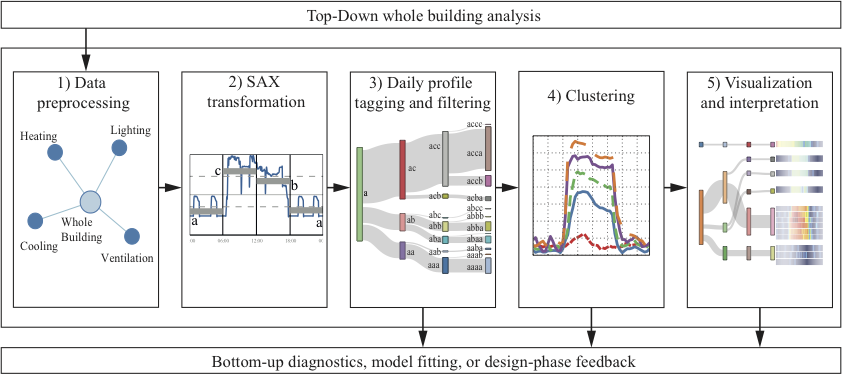
\includegraphics[width=1\columnwidth]{figures/ClusteringProcessDiagram_V4/ClusteringProcessDiagram_V4}
\caption{Diagram of the five steps in the \emph{DayFilter} (from \citep{miller_automated_2015})
\label{fig:process}%
}
\end{center}
\end{figure}

As in any data mining approach, data preprocessing is an important step to clean and standardize the data. In the proposed method, extreme point measurements are removed that fall outside of three standard deviations, 3$\sigma$, of the mean, $\mu$, of the selected univariate data stream $x(t)$. The data are then normalized to create a dataset, $Z(t)$ with an approximate 0 mean and a standard deviation of close to 1 \citep{goldin_similiarity_1995}:

\begin{equation}
Z(t)=\frac{x(t) -\mu}{\sigma}
\end{equation}
% ,i \in N$$

In the second step, $Z(t)$ is transformed into a symbolic representation using SAX. It is one of the many means of representing time-series data to enhance the speed and usability of various analysis techniques. SAX is a type of Piecewise Aggregate Approximation (PAA) representation developed by Keogh et. al and it has been used extensively in numerous applications \citep{lin_experiencing_2007}. 

In brief, the SAX transformation is as follows. The normalized time-series, $Z(t)$, is first broken down into $N$ individual non-overlapping subsequences. This step is known as \emph{chunking}, and the period length $N$ is based on a context-logical specific period \citep{lin_visualizing_2005}. In this situation, $N$ is chosen as 24 hours due to the focus on daily performance characterization.  Each chunk is then further divided into $W$ equal sized segments. The mean of the data across each of these segments is calculated and an alphabetic character is assigned according to where the mean lies within a set of vertical breakpoints, $B=\beta_1,...,\beta_{a-1}$. These breakpoints are calculated according to a chosen alphabet size, $A$, to create equiprobable regions based on a Gaussian distribution, as seen in Table~\ref{fig:SAXBreakpoints}.

\begin{figure}[ht!]
\begin{center}
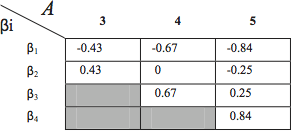
\includegraphics[width=0.42\columnwidth]{figures/SAXBreakpoints/SAXBreakpoints}
\caption{Example breakpoint lookup table from Keogh et. al \citep{keogh_hot_2005} for $A$ = 3, 4, 5 calculated from a Gaussian distribution \citep{miller_automated_2015}
\label{fig:SAXBreakpoints}%
}
\end{center}
\end{figure}

Based on a chosen value of $W$ segments and alphabet size $A$, each $N$ size window is transformed into a SAX \emph{word}. An example of this process is seen in Figure~\ref{fig:SAXWord}. This example shows two daily profiles which are converted to the SAX words, \emph{acba} and \emph{abba}. The SAX word is useful from an interpretation point of view in that each letter corresponds consistently to a subsequence of data from the daily profile. For example, the first letter explains the relative performance for the hours of midnight to 6:00 AM. Therefore if the size of $A$ is set to 3, a SAX word whose first letter is $a$ would have low, $b$ would indicate average, and $c$ would correspond to high consumption. Larger sizes of $A$ would create SAX words with a more diverse range of characters and would capture more resolution magnitude-wise.

\begin{figure}[ht!]
\begin{center}
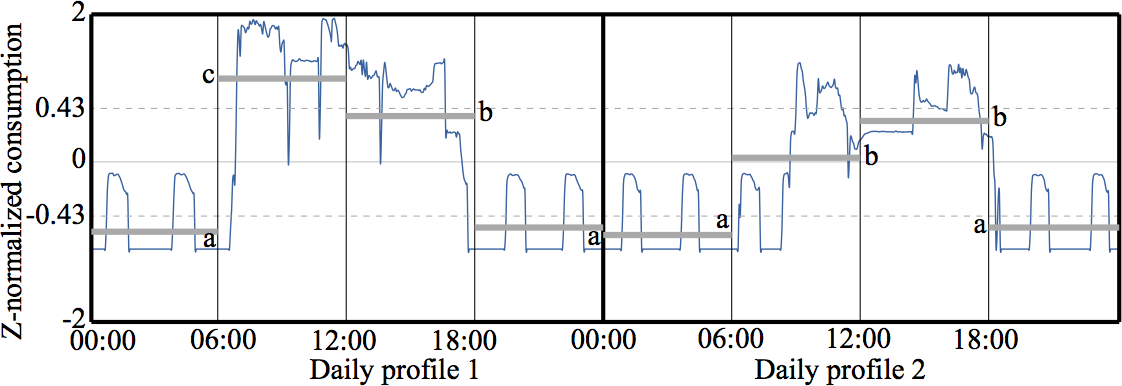
\includegraphics[width=0.7\columnwidth]{figures/SAXCreationV2/SAXCreationV2}
\caption{SAX word creation example (based on figure from Keogh et. al \citep{keogh_hot_2005}) of two days of 3 minute frequency data, parameters are $N$=480, $W$=4, and $A$ = 3 and the generated representative word for daily profile 1 is \emph{acba} and daily profile 2 is \emph{abba} (from \citep{miller_automated_2015})
\label{fig:SAXWord}%
}
\end{center}
\end{figure}

The individual subsequences, $N$, are not normalized independently. This particular decision is divergent from the generalized shape-based discord approaches and is because, at this level of analysis and the context of building performance data, there is interest in discovering interesting subsections based on both magnitude and shape. 
% used with permission from Keogh et. al \citep{Keogh:2005wd}.

The targeted benefits of using SAX in this scenario are that discretization uniformly reduces the dimensionality and creates sets of words from the daily data windows. This transformation allows the use of hashing, filtering, and clustering techniques that are commonly used to manipulate strings \citep{lin_experiencing_2007}. 

Once the SAX words are created, each pattern is visualized and tagged as either a motif or discord. The results of applying the SAX process to a two-week sample power dataset are shown in Figure~\ref{fig:saxcreation}. The diagram shows how each daily chunk of high-frequency data is transformed into a set of SAX characters. In this example, an alphabet size, $A$, of 3 and a subsequence period count, $W$, of 4 are used for each character aggregating the data from 6 hours of each profile. These parameters are the same as used in the more simplified two-day example from Figure~\ref{fig:SAXWord}

\begin{figure}[ht!]
\begin{center}
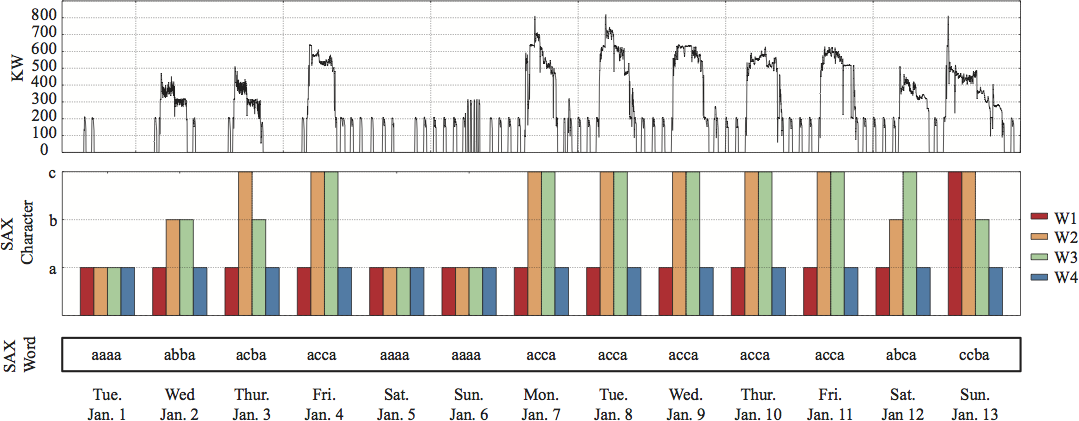
\includegraphics[width=1\columnwidth]{figures/SAXWordExample_BarLine/SAXWordExample_BarLine}
\caption{Creation of SAX words from daily non-overlapping windows: W1: 00:00-06:00, W2: 06:00-12:00, W3: 12:00-18:00, W4: 18:00-24:00. Time series data is transformed according to a SAX character creation and then as a string, or SAX word \citep{miller_automated_2015}
\label{fig:saxcreation}%
}
\end{center}
\end{figure}

Figure~\ref{fig:saxdiscordsankey} visualizes the frequency of the SAX strings and substrings in the form of an augmented suffix tree. Suffix trees have been an integral part of string manipulation and mining for decades \citep{weiner_linear_1973}. Augmented suffix trees enable a means of visualizing the substring patterns to show frequency at each level. This figure incorporates the use of a Sankey diagram to visualize the tree with each substring bar height representing the number of substring patterns existing through each window of the day-types. The more frequent patterns are categorized as \emph{motifs} or patterns which best describe the average behavior of the system. One can see the patterns with the lower frequencies and their indication as \emph{discords} or subsequences that are least common in the stream.  

Heuristically, a decision threshold is set to distinguish between motifs and discords. This threshold can be based on the word frequency count for each pattern as a percentage of the number of all observations. This threshold can be tuned to result in a manageable number of discord candidates to be further analyzed. More details about setting this limit will be discussed the applied case studies.

% The extracted SAX words are grouped according to frequency and a threshold is chosen to differentiate the profiles to consider as motif candidates or as low-frequency day types to tag for further investigation.

In the two-week example, this process yields two patterns which have a frequency greater than one and thus are the motif candidates. A manual review of the data confirms that those patterns match with an expected profile for a typical weekday ($acca$) and weekend ($aaaa$). The less frequent patterns are tagged as discords and can be analyzed in more detail. In this case, it can be determined that the patterns $abba$, $abca$, and $acba$, despite being infrequent, are not abnormal due to the occupancy schedule for those particular days. Pattern $ccba$, however, is not explainable within the scheduling and is due to a fault causing excessive consumption in the early morning hours.

This step leads into the next phase of the process focused on further aggregating the motif candidates of the dataset. The size and number of potential motif filtered in this step will give an indication of the number of clusters that will likely pick up the exact structure from the dataset.

\begin{figure}[ht!]
\begin{center}
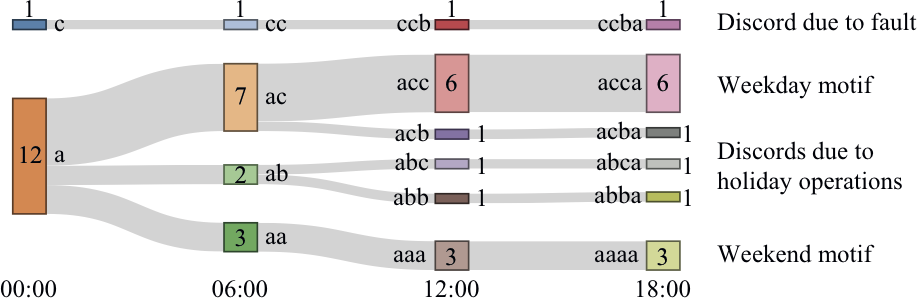
\includegraphics[width=0.84\columnwidth]{figures/DiscordSankeyExample/DiscordSankeyExample}
\caption{Augmented suffix tree of SAX words. Each level from left to right represents the $W1-W4$, the substrings are noted adjacent to each bar, and the bar thickness is proportional to the number of days within each pattern type. The pattern frequency in number of days is noted in this graphic within or just adjacent to each bar. (from \citep{miller_automated_2015})
\label{fig:saxdiscordsankey}%
}
\end{center}
\end{figure}

As the final step, interpretation and visualization are critical for \emph{DayFilter} for a human analyst to visually extract knowledge from the results, and to make decisions regarding further analysis. The \emph{Overview, zoom and filter, details-on-demand} approach \citep{shneiderman_eyes_1996} and the previously mentioned VizTree tool \citep{lin_visually_2004} are used for insight into this process. The hidden structures of building performance data are revealed through the SAX process, and visualization is used to communicate this structure to an analyst. The method uses a modified Sankey diagram to visualize the augmented suffix tree in a way which the count frequency of each SAX word can be distinguished.  Figure~\ref{fig:saxdiscordsankeyheatmap} shows how this visualization is combined with a heat map of the daily profiles associated with each of the SAX words using the same two-week example data from Figures \ref{fig:saxcreation} and \ref{fig:saxdiscordsankey}. The Sankey diagram is rearranged according to the frequency threshold set to distinguish between the motif and discord candidates.

In Figure~\ref{fig:saxdiscordsankeyheatmap}, the discords are shown as the top four days, Jan. 2, 3, 12, and 13 and the remaining days are shown as more frequent potential motifs below. Each daily profile is shown adjacent to the right of the Sankey diagram and is expressed as a color-based heatmap. Each horizontal bar of the heat map is an individual day, and they are grouped according to pattern with the associated legend informing the viewer the magnitude of energy consumption across the day. This visualization is designed to present quickly the patterns arranged according to a sort of hierarchy provided by the suffix tree. One can more easily distinguish seemingly \emph{normal} versus \emph{abnormal} behavior with this combination of visualizations. 

\begin{figure}[ht!]
\begin{center}
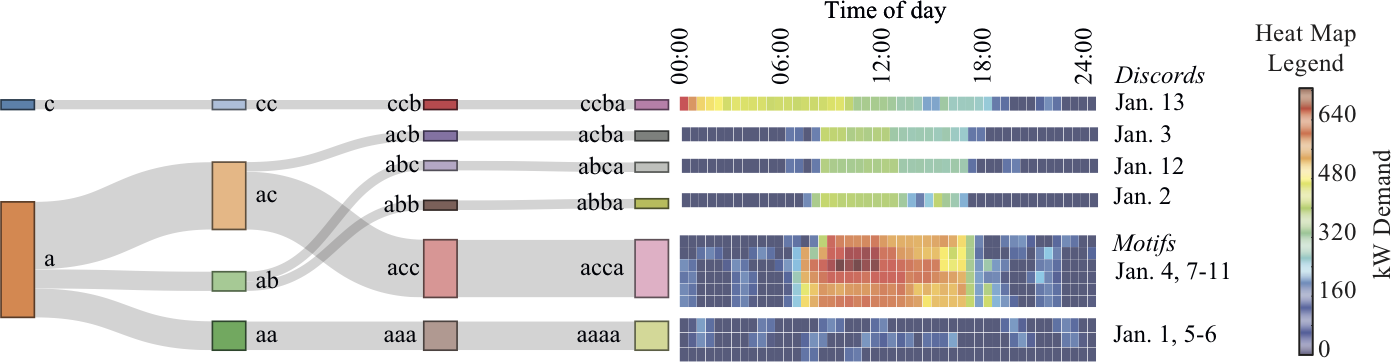
\includegraphics[width=1\columnwidth]{figures/DiscordSankeyExampleWithHeatmapV2/DiscordSankeyExampleWithHeatmapV2}
\caption{Example suffix tree with heatmap from the two week dataset. The sankey diagram illustrates the divisions according to pattern and the general categories of motif vs. discord candidates. Each horizontal line in the heatmap represents a single daily profile to illustrate consumption magnitude of each SAX word. \citep{miller_automated_2015}
\label{fig:saxdiscordsankeyheatmap}%
}
\end{center}
\end{figure}

\emph{DayFilter} is applied on a large energy performance datasets to demonstrate the usability and results in real-life scenarios. The process is applied to a 70,000 square meter international school campus in the humid, tropical climate of Singapore. It was built in 2010 and includes a building management system (BMS) with over 4,000 measured data points taken at 5-minute intervals from the years of 2011-2013 - resulting in close to 800 million records of raw data. This collection includes 120 power meters and 100 water meters in the energy and water management system. The data from this study are a seed dataset in an open repository of detailed commercial building datasets \citep{miller_seed_2014}. 

The chilled water plant electricity consumption is targeted in this case due to its importance in this climate and the potential savings opportunities available through chilled water plant optimization. Measured kilowatt-hour (kWh) and kilowatt (kW) readings were taken from July 12, 2012, to October 29, 2013, with 474 total daily profiles analyzed. Figure~\ref{fig:sankeyheatmap1} illustrates a Sankey diagram with a heat map of the output of the \emph{DayFilter} process with parameters set to $A$=3 and $W$=4. The discord and motif candidates are separated in this case according to a decision threshold which quantifies a discord as a day-type with a frequency count less than 2\% of total days available. This distinction results in 39 days with patterns tagged as discord candidates, which is 8.2\% of the total days in the dataset. 

\begin{figure}[ht!]
\begin{center}
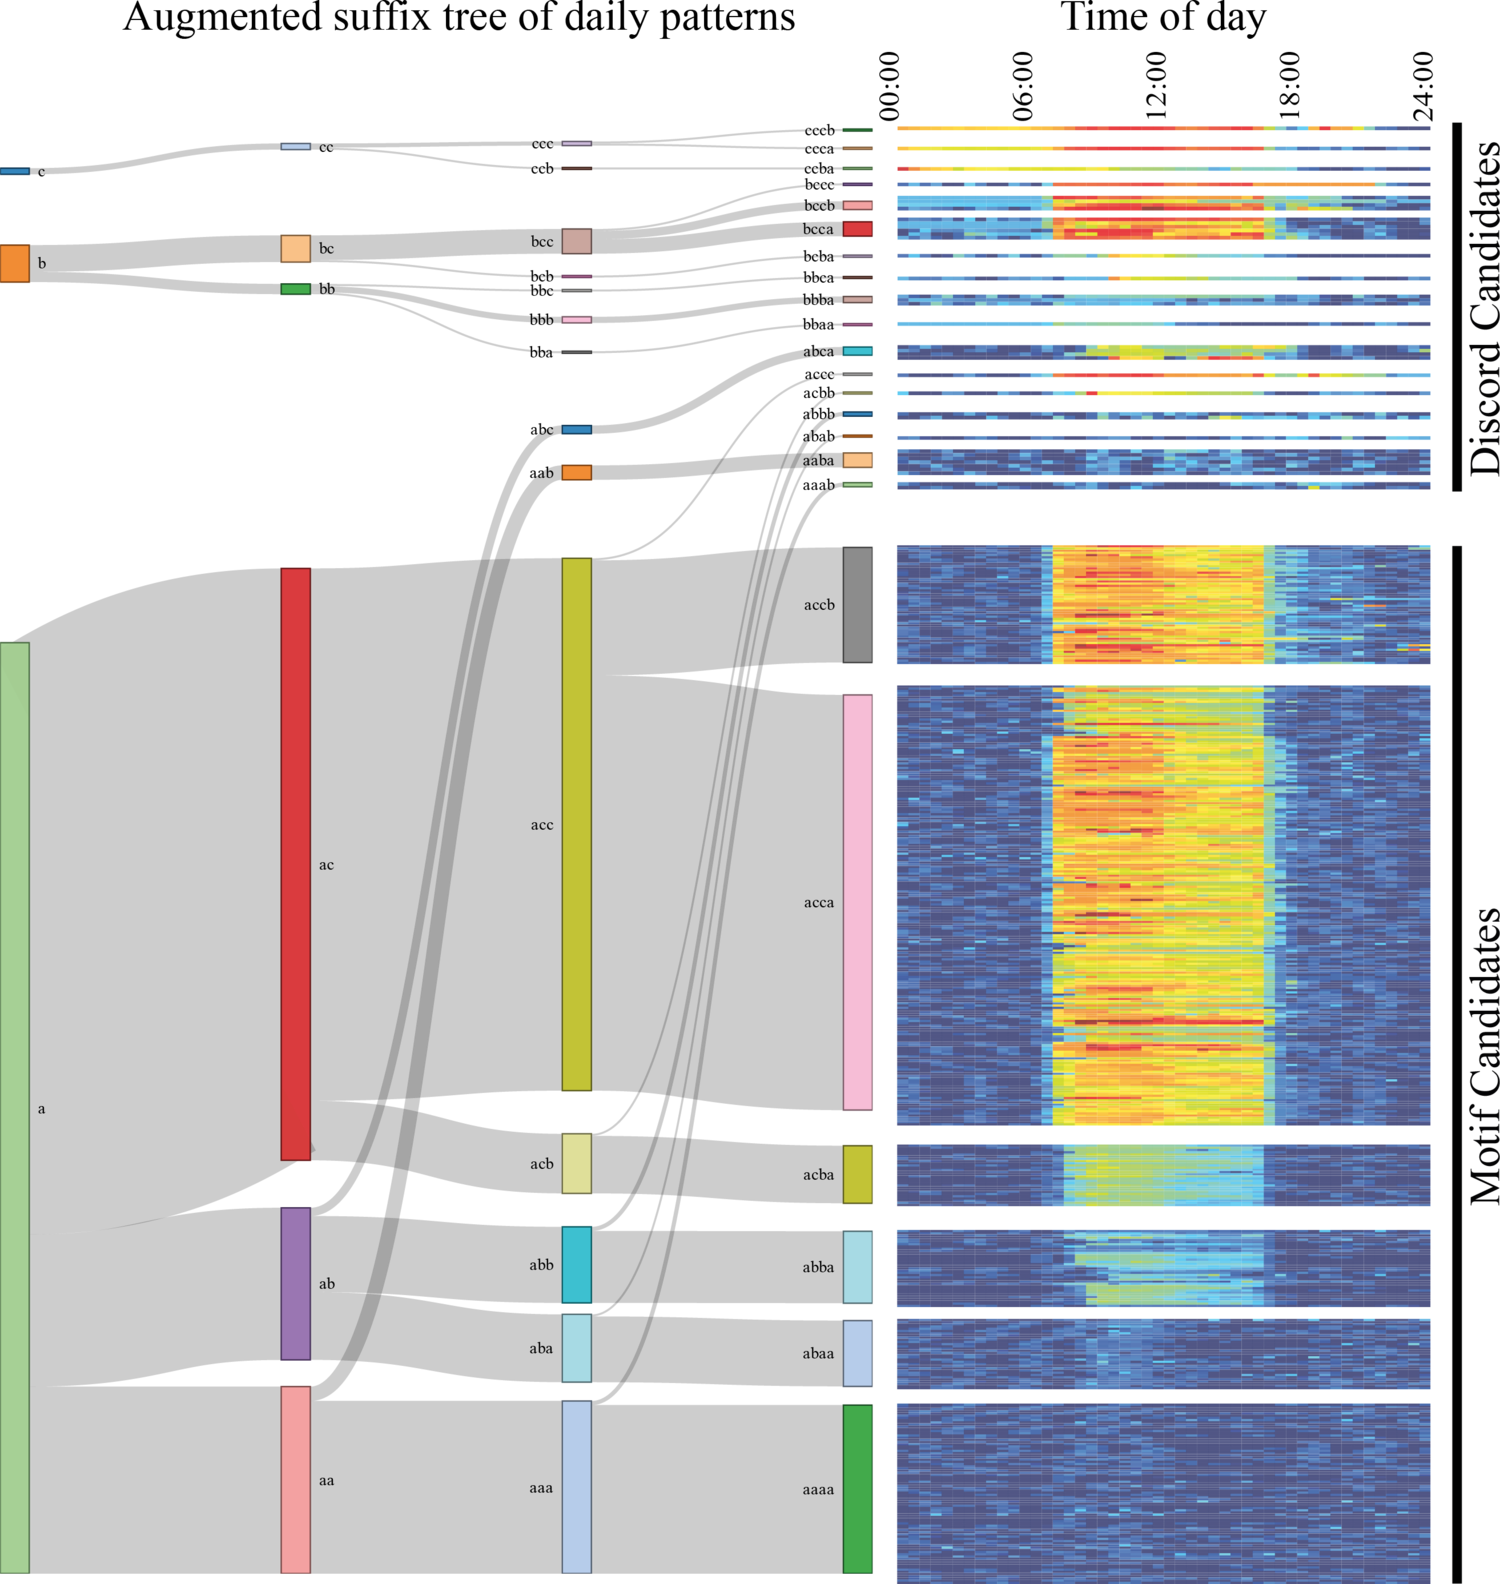
\includegraphics[width=1\columnwidth]{figures/UWC_Chiller_SankeyHeatmapV2/UWC_Chiller_SankeyHeatmapV2}
\caption{Cooling electricity consumption representation of the day-types from the DayFilter process \citep{miller_automated_2015}
\label{fig:sankeyheatmap1}%
}
\end{center}
\end{figure}

In general, there are six primary motif candidates with two candidates appearing to be typical weekday types, two holiday or half-capacity types, and two-weekend unoccupied types. Pattern $aaaa$ and $abaa$ are predominantly flat profiles common to non-occupied cooling consumption. Patterns $abba$ and $acba$ are representative of days in which school is out of session, but staff still occupies the office spaces. Pattern $acca$ represents a regular full-occupied school day, and it is by far the most common with 202 days tagged out of 474. Pattern $accb$ is similar to $acca$ with slightly more use in the late afternoon and early evening. This phenomenon is due to extracurricular activities planned outside the normal operating schedule of the facility.

For characterization, a metric is developed from the \emph{DayFilter} process that approximates the presence of motifs and discords. This metric is a daily frequency calculation of each day's pattern count versus the total number of days. An example of this metric is seen in Figure \ref{fig:dayfilter_single}.

\begin{figure}[ht!]
\begin{center}
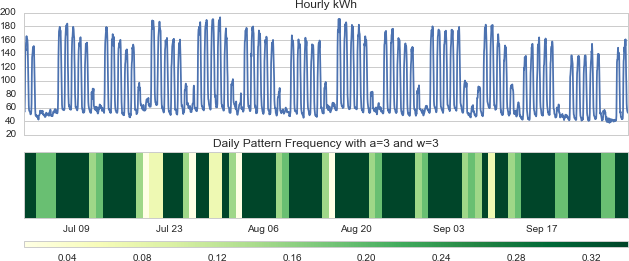
\includegraphics[width=1\columnwidth]{figures/dayfilter_example1/dayfilter_example1}
\caption{Single building example of daily pattern frequency using \emph{DayFilter}, a=3 and w=3
\label{fig:dayfilter_single}%
}
\end{center}
\end{figure}

\subsection{Pattern Specificity}
\label{sec:patternspec}

Another way to leverage SAX to characterize the case study data is to use it to extract which patterns are most indicative of a particular building use type. This information is obtained using the SAX-VSM process pioneered by Senin and Malinchik that uses SAX and Vector Space Model technique from the text mining field \citep{Senin_2013}. Conventionally this method is utilized as a classification model to predict which class a certain time-series belongs. A by-product of the process is that the subsequences of each data stream are assigned a metric indicating their specificity. Pattern specificity is a concept that quantifies how well a meter \emph{fits within its class}. This technique is used to determine whether a building is operating similar to other supposed peer buildings of the same type.

The SAX-VSM process begins with the SAX word creation, similar to \emph{DayFilter} as shown in Figure \ref{fig:saxcreation}. However, the key difference is that the conventional SAX process extracts word patterns from overlapping windows as opposed to simply \emph{chunking} each daily profile. Each data stream within a particular class of a training data set is converted to SAX words using the same input variables of alphabet size, $A$, and subsequence period count, $W$. In addition, a $P$ variable is chosen to indicate the size of the sliding window. With SAX-VSM, all of the SAX words for a certain use type class, such as Offices, are then combined into a large Bag of Words (BOG) representation called a corpus, and then used to build a term frequency matrix. This model is then used to calculate a $tf*idf$ weight coefficient, which is the product of the term frequency ($tf$) and the inverse document frequency ($idf$). The term frequency is a logarithmically scaled metric based on the incidence of a pattern in the BOG. The inverse document frequency is computed as the log of the ratio of the number of classes to the number of bags where each pattern occurs \citep{Manning}. Once this matrix of weight vectors is computed, the cosine similarity of an individual data stream can be calculated to determine how similar to each class it is. 

\begin{figure}[ht!]
\begin{center}
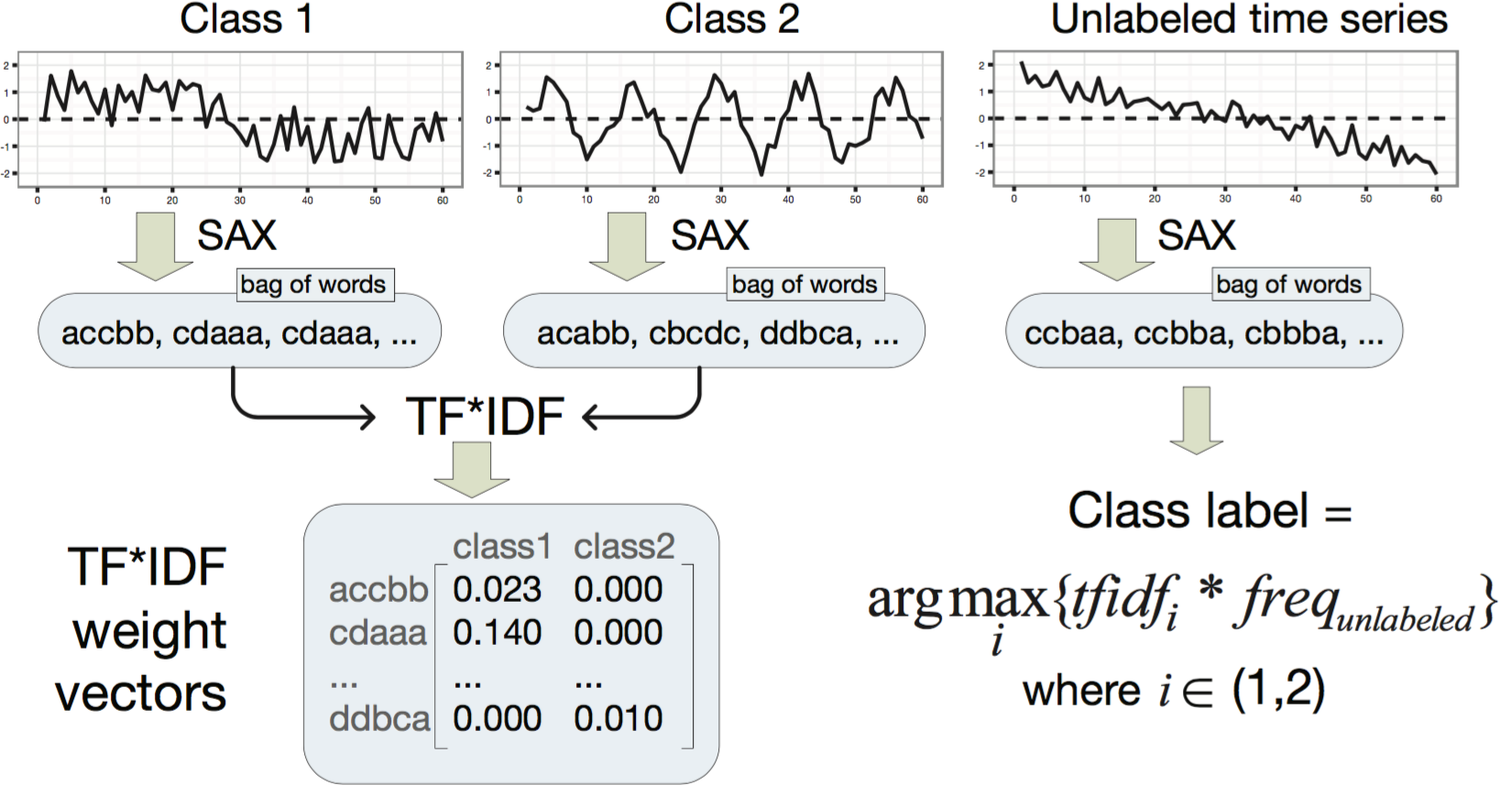
\includegraphics[width=0.98\columnwidth]{figures/jmotif/jmotif}
\caption{Overview of SAX-VSM algorithm: first, labeled time series are converted into bags of words using SAX; secondly, $tf*idf$ statistics is computed resulting in a single weight vector per training class. For classification, an unlabeled time series is converted into a term frequency vector and assigned a label of a weight vector which yields a maximal cosine similarity value (figure and caption used with permission from \citep{senin_sax-vsm:_2013}).
\label{fig:saxvsm_overview}%
}
\end{center}
\end{figure}

In this study, the goal is not to use SAX-VSM to classify each data stream, but to extract instead temporal features that can be used to characterize them. Thus, the in-class cosine similarity is calculated for each building's data set as compared to the class it was assigned. This process is not conventional from the classification sense as it is considered over-fitting due to all samples being included in the training set. This situation is tolerated in this analysis as it is desired to quantify only how much the patterns of use for a building compare to those of its labeled \emph{peers}.

The specificity metric for each data stream is calculated for each sliding window by subtracting all other $tf*idf$ weights for each pattern from the in-class weighting. 

\begin{figure}[ht!]
\begin{center}
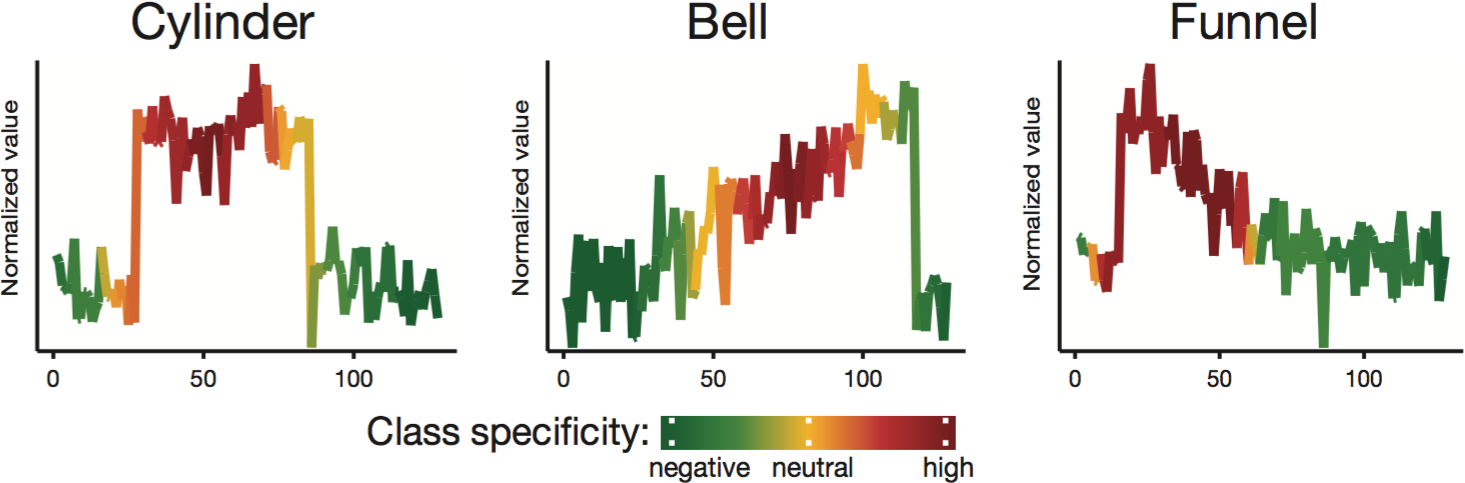
\includegraphics[width=1\columnwidth]{figures/jmotif_tfidfspec/jmotif_tfidfspec}
\caption{An example of the heat map-like visualization of subsequence \emph{importance} to a class identification. Color value of each point was obtained by combining $tf*idf$ weights of all patterns which cover the point. The highlighted class specificity corresponds to a sudden rise, a plateau, and a sudden drop in Cylinder; to a gradual increase in Bell; and to a sudden rise followed by a gradual decline in Funnel (figure and caption used with permission from \citep{senin_sax-vsm:_2013})
\label{fig:specificity_example}%
}
\end{center}
\end{figure}

The specificity calculation process is implemented on each of the building test data sets. A single building example of this process is seen in Figure \ref{fig:dailyspecificity_single}. This building is within the \emph{Office} use-type classification; thus the color spectrum indicates how precise each subsequence is to this building's behavior as an office as compared to the entire training data set. This example is using the input metrics of $a=8$, $p=8$, and $w=24$ to capture the specificity of daily patterns. These parameters settings include the use of a 24-hour sliding window that is divided into eight segments of three hours length, and the normalized magnitude assigns a symbol from a range of eight letters, $a,b,c,d,e,f,g,h$.

\begin{figure}[ht!]
\begin{center}
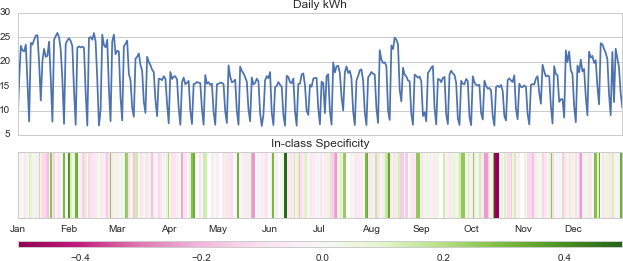
\includegraphics[width=1\columnwidth]{figures/jmotif_alldatatrained_dailyspecificity_example_24_8_8/jmotif_alldatatrained_dailyspecificity_example_24_8_8}
\caption{Single building example of daily in-class specificity, a=8, p=8, and w=24 for an office building. Positive specificity indicates behavior that is characteristic of a certain class, while negative values indicates behavior of a different class.
\label{fig:dailyspecificity_single}%
}
\end{center}
\end{figure}

The specificity calculation process also implemented using input parameters designed to capture patterns of weekly behavior. In this situation, the input metrics of $a=6$, $p=14$, and $w=168$ are chosen to capture this behavior. These parameters settings model a 168-hour sliding window (one week) that is divided into 14 segments of 12 hours length, and the normalized magnitude assigns a symbol from a range of six letters, $a,b,c,d,e,f$. A single building example is seen in Figure \ref{fig:weeklyspecificity_single}. This building is also within the \emph{Office} use-type classification; thus the color spectrum indicates how precise each weekly subsequence is to this building's behavior as an office as compared to the entire training data set.

\begin{figure}[ht!]
\begin{center}
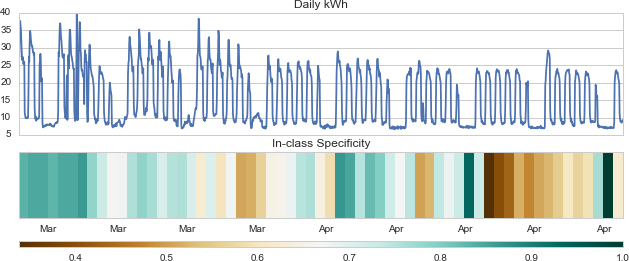
\includegraphics[width=1\columnwidth]{figures/jmotif_alldatatrained_dailyspecificity_example_168_6_14/jmotif_alldatatrained_dailyspecificity_example_168_6_14}
\caption{Single building example of weekly in-class specificity, a=x, w=X, and p=X
\label{fig:weeklyspecificity_single}%
}
\end{center}
\end{figure}

\subsection{Long-term Pattern Consistency}
\label{sec:patternconsistency}

Breakout detection screening is a process in which each data stream is analyzed according to the tendency to shift from one performance state to another with a transition period in between. This metric is used in this context to quantify long-term pattern consistency, and much of the explanation and graphics in this section are from a previous study \citep{miller_forensically_2015}. Breakout detection is a type of change point detection that determines whether a change has taken place in a time series dataset. Change detection enables the segmentation of the data set to understand the nonstationarities caused by the underlying processes and is used in multiple disciplines involving time-series data such as quality control, navigation system monitoring, and linguistics \citep{basseville_detection_1993}. Breakout detection is applied to temporal performance data to understand general, continuous areas of performance that are similar and the transition periods between them.

In this process, an R programming package, \emph{BreakoutDetection}, is utilized, which is also developed by Twitter to process time-series data related to social media postings\footnote{https://github.com/twitter/BreakoutDetection}. This package uses statistical techniques which calculate a divergence in mean and uses robust metrics to estimate the significance of a breakout through a permutation test. The specific technical details of the breakout detection implementation can be found in a study by James et al. \citep{james2014leveraging}. \emph{BreakoutDetection} uses the E-Divisive with Medians (EDM) algorithm, which is robust amongst anomalies and can detect multiple breakouts per time series. It can identify the two types of breakouts, mean shift and ramp up. Mean shift is a sudden jump in the average of a data stream, and ramp up is a gradual change of the value of a metric from one steady state to another. The algorithm has parameter settings for the minimum number of samples between breakout events that allows the user to modulate the amount of temporal detail.

The goal in using breakout detection for building performance data is to find directly when macro changes occur in sensor data stream. This discovery is particularly exciting in weather-insensitive data to understand when modifications are made to the underlying system in which performance is being measured. Figure \ref{fig:breakout_single} data from a single building data stream. Each color represents a group of continuous, steady-state operation and each change in color is, thus, a breakout. These breakouts could be the result of schedule or control sequence modifications, systematic behavior changes, space use type changes, etc. Creation of diversity factor schedules should target data streams which have few breakouts and the data between breakouts is the most applicable for model input. One parameter setting for breakout detection is the minimum breakout size threshold. This parameter prevents breakouts from being detected to close together, thus capturing potentially noisy behavior for the particular data set.

\begin{figure}[ht!]
\begin{center}
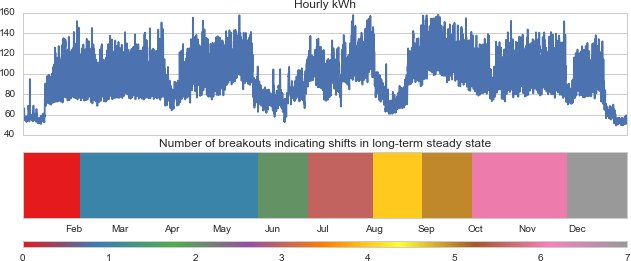
\includegraphics[width=1\columnwidth]{figures/breakout_example/breakout_example}
\caption{Single building example of breakout detection to test for long-term volatility in an university dormitory building. A minimum threshold of 30 days is chosen in this case, which explains the lack of threshold shift in April, a break that may be attributed to spring break for this building
\label{fig:breakout_single}%
}
\end{center}
\end{figure}

\section{Implementation and Discussion}
\label{sec:patternbaseddiscussion}

Figure \ref{fig:dayfilter_all} shows this pattern frequency metric as applied to all the case study buildings. One will notice that there is a range of pattern frequencies occurring across each of the building use types. Offices and Primary/Secondary Classrooms seem to have larger regions of darker, more consistent behaviour. Labs and Classrooms seem to be more volatile across the time ranges.

\begin{figure}[ht!]
\begin{center}
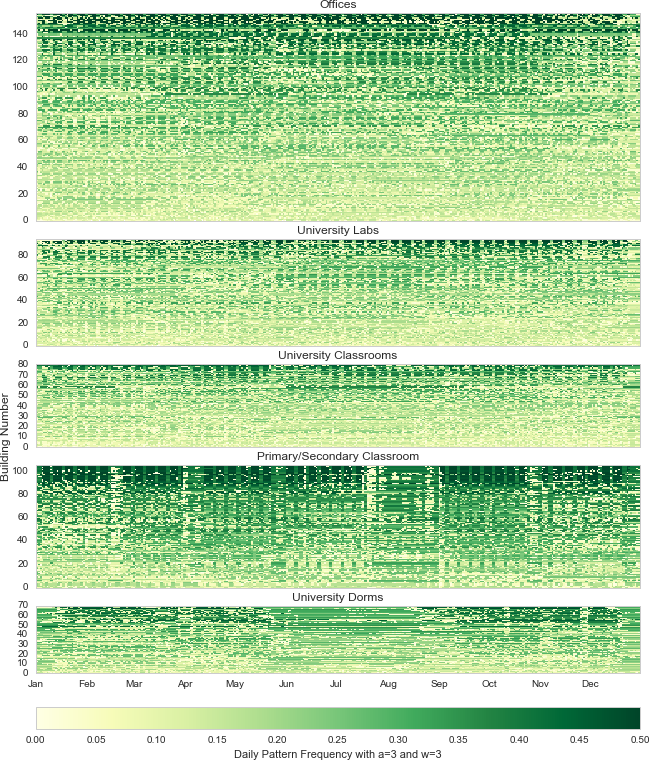
\includegraphics[width=1\columnwidth]{figures/dayfilter_heatmap/dayfilter_heatmap}
\caption{Heatmap of daily pattern frequencies using \emph{DayFilter} with a=3 and w=3
\label{fig:dayfilter_all}%
}
\end{center}
\end{figure}

Figure \ref{fig:dailyspecificity_all} illustrates this process applied to all 507 case studies as divided amongst the use types. Clear differences in patterns across the time ranges are visible for each of the building use types. Offices, university laboratories, and university classrooms all seem to have similar phases of specificity at similar times of the year, while dorms and primary/secondary schools are often differentiated by their breaks.

\begin{figure}[ht!]
\begin{center}
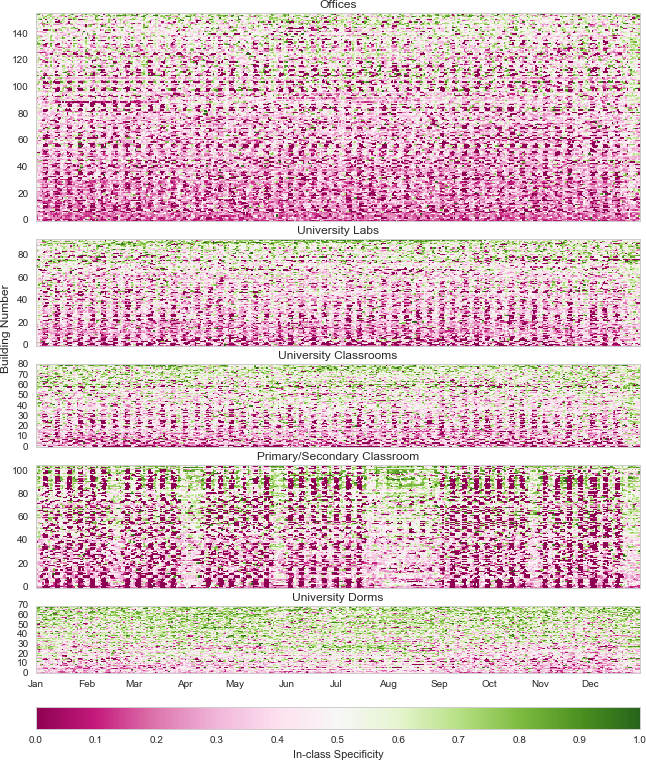
\includegraphics[width=1\columnwidth]{figures/jmotif_inclassspec_allbuildings_heatmap_24_8_8/jmotif_inclassspec_allbuildings_heatmap_24_8_8}
\caption{Heatmap of in-class specificity with p=24, a=8, w=8
\label{fig:dailyspecificity_all}%
}
\end{center}
\end{figure}

Figure \ref{fig:weeklyspecificity_all} illustrates weekly specificity as applied to all the buildings. The transition between specific and non-specific patterns is smoother in this case due to the weekly time range. It is also apparent that the most distinct behavior patterns for each building use type are correlated to when that particular building has behavior related to lower occupancy such as summer breaks or holiday periods. These phenomena need to be somewhat consistent across all the buildings within a classification for it to indicate specificity.  

\begin{figure}[ht!]
\begin{center}
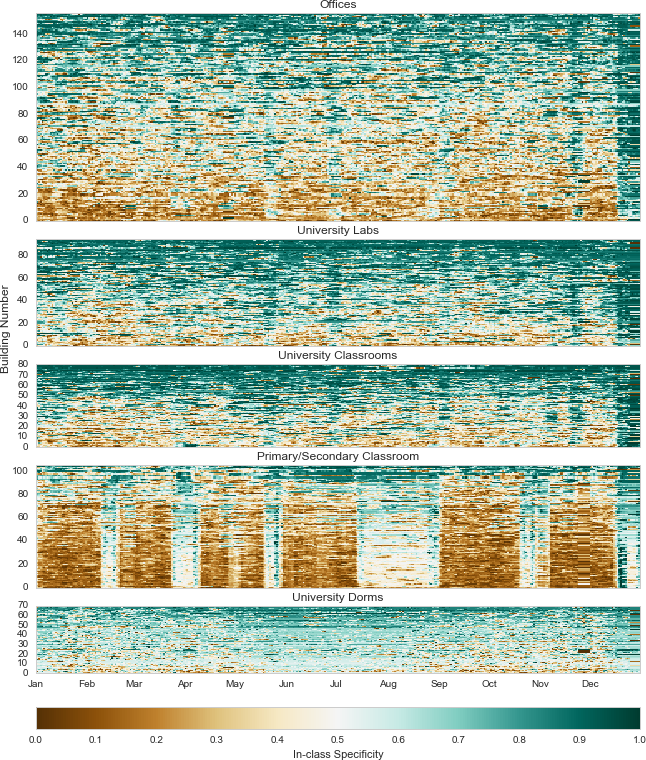
\includegraphics[width=1\columnwidth]{figures/jmotif_inclassspec_allbuildings_heatmap_168_6_14/jmotif_inclassspec_allbuildings_heatmap_168_6_14}
\caption{Heatmap of in-class specificity with p=168, a=6, w=14
\label{fig:weeklyspecificity_all}%
}
\end{center}
\end{figure}


Figure \ref{fig:breakout_heatmap} illustrates breakout detection across the building use types in this study. This implementation uses the same input parameter of a 30 day minimum between breakouts. One notices somewhat of consistency amongst offices, labs, and classrooms regarding the distribution of breakout numbers, while university dormitories and primary/secondary classrooms have a noticeably higher number of breakouts across the range of behavior.

\begin{figure}[ht!]
\begin{center}
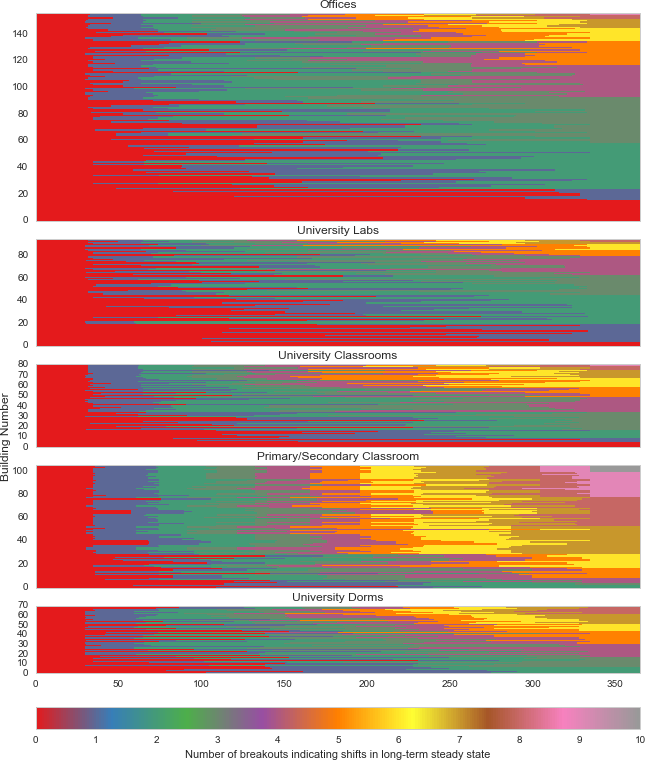
\includegraphics[width=1\columnwidth]{figures/breakouts_heatmap/breakouts_heatmap}
\caption{Heatmap of breakout detection on all case studies
\label{fig:breakout_heatmap}%
}
\end{center}
\end{figure}
